\documentclass[11pt]{exam}

\oddsidemargin=0.25truein \evensidemargin=0.25truein
\topmargin=-0.5truein \textwidth=6.0truein \textheight=8.75truein

%\RequirePackage{graphicx}
\usepackage{comment}
\usepackage{verbatim}
\usepackage{booktabs}
\usepackage{graphicx}
\usepackage{hyperref}
\urlstyle{rm}   % change fonts for url's (from Chad Jones)
\hypersetup{
    colorlinks=true,        % kills boxes
    allcolors=blue,
    pdfsubject={ECON-UB233, Macroeconomic foundations for asset pricing},
    pdfauthor={Dave Backus @ NYU},
    pdfstartview={FitH},
    pdfpagemode={UseNone},
%    pdfnewwindow=true,      % links in new window
%    linkcolor=blue,         % color of internal links
%    citecolor=blue,         % color of links to bibliography
%    filecolor=blue,         % color of file links
%    urlcolor=blue           % color of external links
% see:  http://www.tug.org/applications/hyperref/manual.html
}

\renewcommand{\thefootnote}{\fnsymbol{footnote}}
\newcommand{\var}{\mbox{\it Var\/}}

%\printanswers

% document starts here
\begin{document}
\parskip=\bigskipamount
\parindent=0.0in
\thispagestyle{empty}
{\large ECON-UB 233 \hfill Dave Backus @ NYU}

\bigskip\bigskip
\centerline{\Large \bf Lab Report \#5: Options \& Volatility}
\centerline{(Started: August 20, 2011; Revised: \today)}

\bigskip
{\it Due at the start of class.
You may speak to others, but whatever you hand in should be your own work.}

\begin{questions}

\begin{solution}
Answers follow.  See Matlab code at the end for calculations.
\end{solution}

%-----------------------------------------------------------------------
\question (BSM formula)
We'll examine the BSM formula in some purely theoretical numerical examples.
In what follows, the current price of the underlying
is 100, the option maturity is one year, and the one-year bond price is 0.98.
\begin{parts}
\part If volatility $\sigma = 0.10$,
what are the prices of call options at strike prices
of 90, 100, and 110?
\part What are the prices of put options with the same strikes?
\part If volatility rises to $\sigma = 0.15$,
what happens to the prices of calls?
\part For strikes of 90, 100, and 110,
graph the call price against volatility $\sigma$
using a grid between (roughly) 0.01 and 0.50.
(This gives you three lines, one for each strike.)
How do call prices vary with volatility?
Does the pattern vary with the strike price?
\part For a strike of 110 and a call price of 2.00,
what is the implied value of $\sigma$?
\end{parts}

\begin{solution}
\begin{enumerate}
\item[(a,b,c)] Answers below (more accuracy than you need).
Put prices were computed from calls using put-call parity.
See Matlab code for details.
%
\begin{center}
\begin{tabular}{rrrr}
\toprule
Strike      &  Call (0.10) & Call (0.15) & Put (0.10) \\
\midrule
   90.0000  & 12.2691  & 13.3828  &  0.4691  \\
  100.0000  &  5.0281  &  6.9722  &  3.0281  \\
  110.0000  &  1.3584  &  3.0726  &  9.1584  \\
\bottomrule
\end{tabular}
\end{center}

\item [(d)] You can see the results in the figure below.
Call prices increase with volatility in all cases.
(Puts, too, for that matter.)
For at-the-money options, the relation is linear.
For others, there's some curvature to it.
You can't see it in the figure, but it's S-shaped.
You can see how this works if you look at the formula for
the derivative (the ``vega''), but that's more than we need here.

\begin{center}
%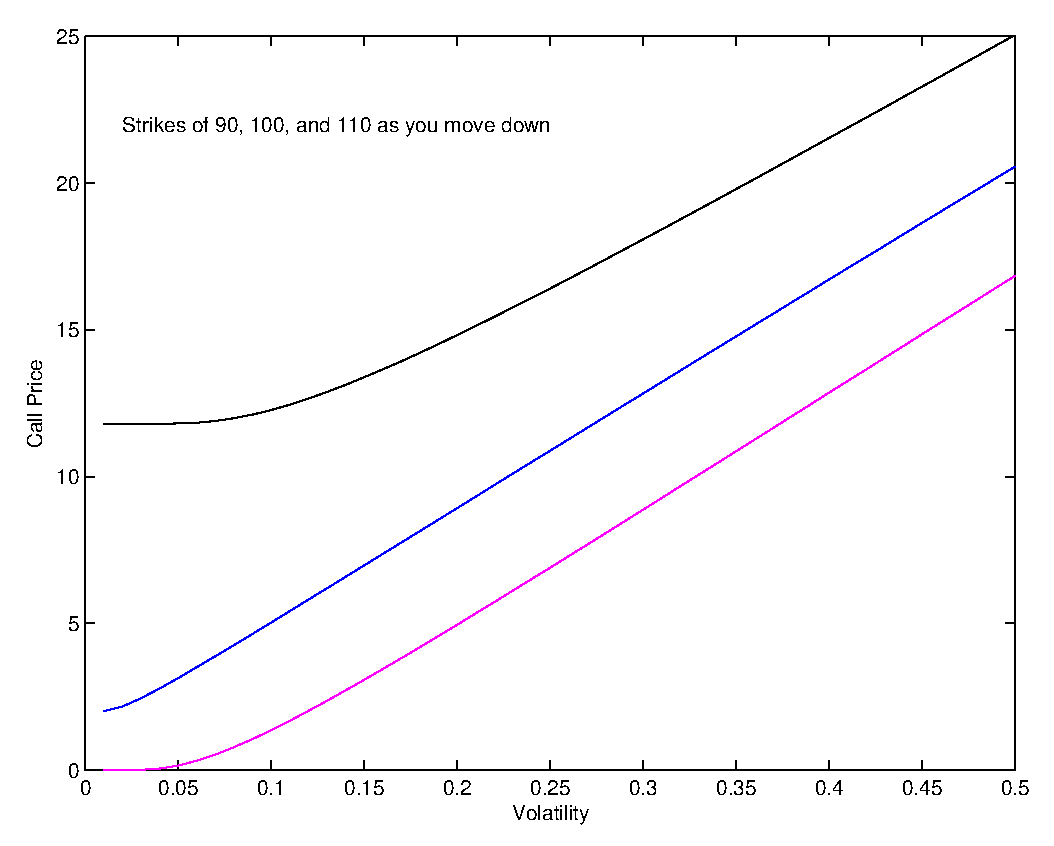
\includegraphics[width=4in]{../Matlab/hw5_q1d.eps}
\end{center}

\item[(e)] From the values computed for the figure, $\sigma = 0.12$ is about it.

\end{enumerate}
\end{solution}


%-----------------------------------------------------------------------
\question (volatilities on S\&P 500 E-mini options)
For the S\&P 500 E-mini options,
the prices of options are more conveniently expressed in
terms of their implied volatilities.
We'll compute them here for quotes reported on March 15, 2012:

\begin{center}
\tabcolsep=0.15in
\begin{tabular}{lcccc}
\toprule
      &  \multicolumn{2}{c}{Call Price} &  \multicolumn{2}{c}{Put Price}  \\
Strike    &  Bid & Ask &  Bid & Ask  \\
\midrule
1340  & 82.50 & 85.75 & 28.25 & 30.25 \\
1350  & 75.25 & 78.25 & 30.75 & 32.75 \\
1360  & 68.00 & 71.00 & 33.25 & 35.50  \\
1370  & 61.25 & 64.00 & 36.25 & 38.75 \\
1380  & 54.50 & 57.25 & 39.50 & 42.25 \\
1390  & 48.25 & 50.75 & 43.25 & 45.75  \\
1400  & 42.25 & 44.75 & 47.00 & 50.00  \\
1410  & 36.75 & 39.25 & 51.25 & 54.50   \\
1420  & 31.75 & 33.75 & 56.00 & 59.25 \\
1430  & 27.00 & 29.00 & 61.25 & 64.50  \\
\bottomrule
\end{tabular}
\end{center}
The price of the underlying contract was 1395.75.
The interest rate was essentially zero, so the appropriate bond price was one.
The options expire June 15, so $\tau = 3/12 = 1/4 $.

\begin{parts}
\part Compute ``mid'' quotes as averages of bid and ask.
Use put-call parity to compute call prices from mid puts.
Plot call prices --- bid, ask, and implied by puts ---
against the strike.
How do they compare?

\part Write a program using, say, the secant method
to compute implied volatilities for mid quotes of call options.
Graph them against the strike.
What shape does the resulting ``smile'' have?
What does the shape suggest to you?
\end{parts}

\begin{solution}
\begin{parts}
\part See the figure below.
Call prices computed from mid puts (asterisks)
are within the bid-ask spread for call prices.
%
\begin{center}
%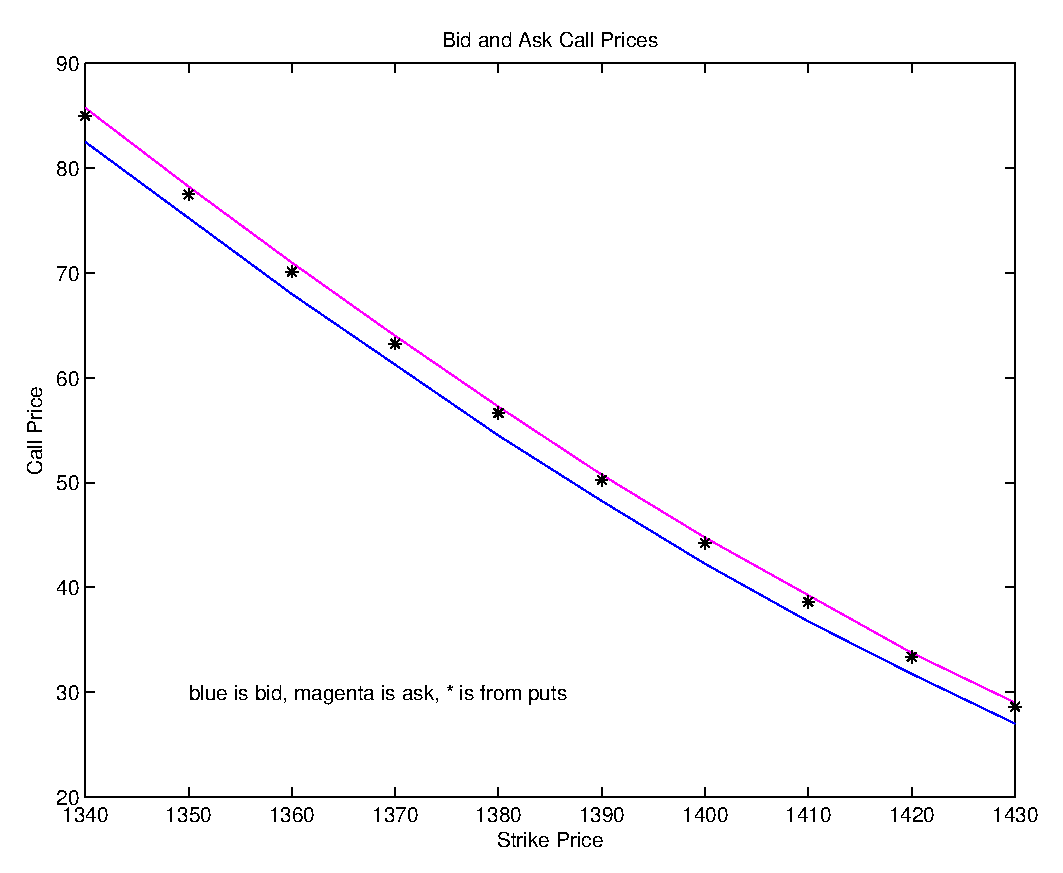
\includegraphics[width=4in]{../Matlab/hw5_q2a.eps}
\end{center}

\part Another figure:
%
\begin{center}
%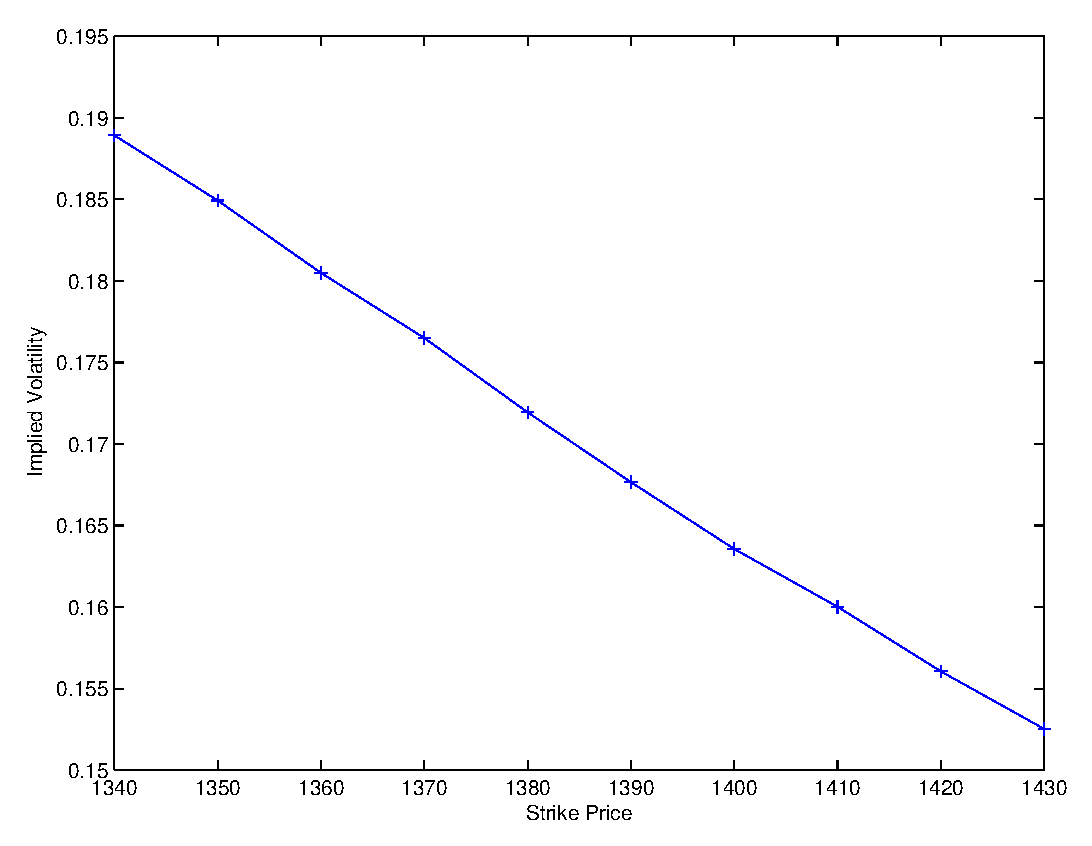
\includegraphics[width=4in]{../Matlab/hw5_q2b.eps}
\end{center}
%
I used the secant method
on $\log(\sigma)$, but the log is probably overkill.
We see that implied vols decline with strike.
That means that prices at low strikes are relatively more expensive than the BSM formula
with constant $\sigma$ would suggest.
This isn't really a smile, but it's what you see for equity index options.
You would also usually see, at least at shorter maturities, some convexity
in the smile that isn't apparent here.
\end{parts}
\end{solution}

\end{questions}

\vfill \centerline{\it \copyright \ \number\year \
NYU Stern School of Business}

%\end{document}

\pagebreak
Matlab program:
\verbatiminput{../Matlab/hw5_s12.m}

\end{document}


%  EXTRA STUFF


